\section{Implementation}
To help us get a better understanding of the development process, we settled on using a software engineering practices called Agile methodology. By using Agile methodology in this project, it helped us to get a better overview of the overall product. The main reason to use agile methodology is that, you can always go back and change the requirements and functionalities of the software while developing. 
In our case we had a stakeholder which is based on the persona, that was mentioned earlier. \newline 
Reflecting on the implementation it gave us alot of knowledge and oppportunities to go back and change the the different functionalities to help us live up to the needs of the stakeholders, to make sure that the software was made for their specific use case, and help us stay in the scope of the project. \newline
To help us manage and optimize the develpoment process, we used Scrum, which is a framework that uses the same priciples as the agile methodology. The use of scrum helped us to stay organized, by splitting the project into smaller parts, to help keep track of what needed to be done.
We decided to split the project into five different sprints and each sprint was about two weeks time. By splitting the project into different sprints, we could get an overview of what needed to be done for that current sprint, while looking forward and seeing what needed to be done in the future. 
While also seeing what did not get done in the current sprint. If a feature was not implemented in the current sprint, we could either delete it or move it to the upcomming sprint, this was very usefull to make sure that all functionalities and requirements where fulfilled.

\subsubsection{Technologies}
To help us develop the system, we decided to use some different software technologies that includes Docker, Node.js, React, OPC-UA. All the listed thing helped us develop the system the way we wanted it.
Docker is a containerization feture that allows us to run several applications in a single container. We decided to use docker to run the OPC-UA client, frontend and backend. By using the containerization technology we could boot the applications simultaneously, instead of running them seperate in their own file. This saved us alot of time and trouble.\newline
The backend is developed in Node.js, which is a javascript package. The reason that we decided to use node.js was because the frontend is developed in React, which also is a javascript package. This helped us to get a secure and easy connection between the frontend and the backned without to much effort. The OPC-UA client is developed in javascript, with a package called node-opcua. This is an open source package that allows connection and communication with an OPC-UA server. \newline
The reason we went with node-opcua instead of the provided MILO package in Java 8, was because, we already decided that we wanted to build in backend and frontend in javascript, and by using node-opcua we could use the same language for the OPC-UA client. This allowed us to establish a secure connections without failures, and it also allows us a better integrity of the system. 
By using javascript for the overall structure of the system, we could ensure that the system is scalable and maintainable in the future. Aswell as not having multiple different programming languages in the system, which can lead to conflics and other problems. \newline

\subsection{Design Implementation}

\subsubsection{Architecture Implementation}
The implementation of the system is based on making a system that is rather easy to maintain and expand on in the future. We decided to use a container to run the backend, frontend and OPC-UA Client. This is done by using a dockerfile, that boots up the different containers.
by doing it this way, we can easiliy maintain and add feutures to the system. It also allows us to live up to the need of the user, where he only needs to click the beer he wants, and then the system will do all the things for him. \newline
To give a better understanding of the system, and the integrity, we made a deployment diagram, that shows how the system is deployed, and how the different components are conncted and talking to each other. \newline

\subsubsubsection{Deployment Diagram}
\begin{center}
    \centering
    \begin{figure}[H]
        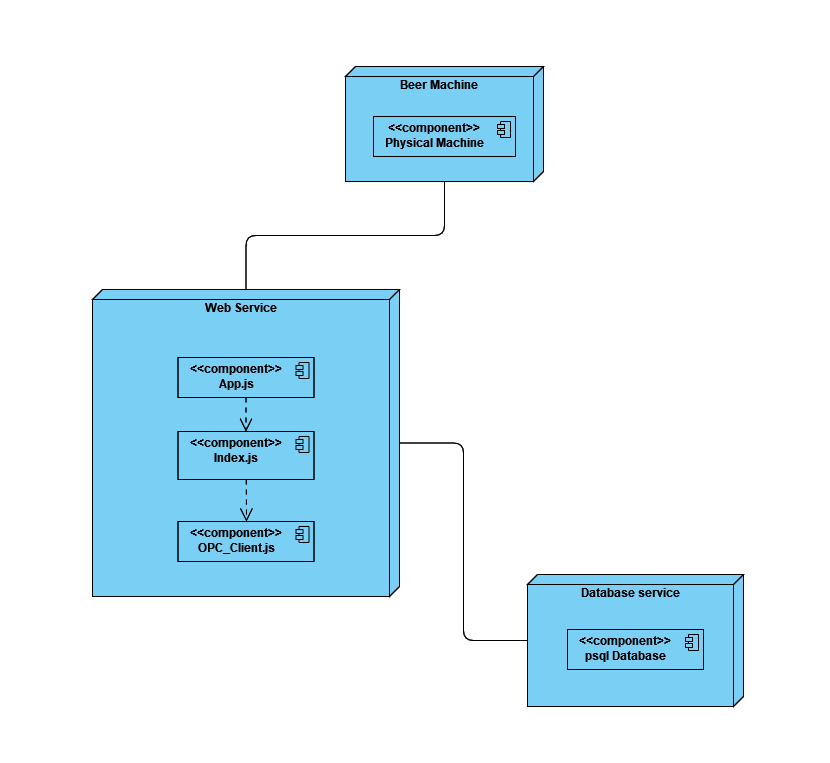
\includegraphics[width=1\textwidth]{img/Deployment_diagram.png}
        \caption{Deployment diagram over the system}
        \label{fig:Deployment_diagram}
    \end{figure}
\end{center}
Figure \ref{fig:Deployment_diagram} shows the deployment diagram of the system. The diagram shows how the different components are conncted and to give a visual understanding of the system. The system is divided into three components, a dockerfile that boots up the backend, frontend and OPCUA-Client, we have the beer machine itself, and lastly the database which enables us to save data that is generated during the brewing process. This data collected can be accesed and help us udnerstand and give improvments to the system. \newline

By deploying the system this way, we can ensure that the system is scalable and maintable in the future. it also enables us to add new features such as new beer recipes, or other things the client may want to help him brew beers. be encapsling the webservice into a container, we can make changes, updates and etc, which helps us reducing the risk of conflics with other parts of the system. \newline

\subsubsubsection{Sequence diagram}

Now that we have declared how the system is being deployed, its important to understand the realations/communication between the different application, in the following sequence diagram, we can see the interation between the application.

\begin{center}
    \centering
    \begin{figure}[H]
        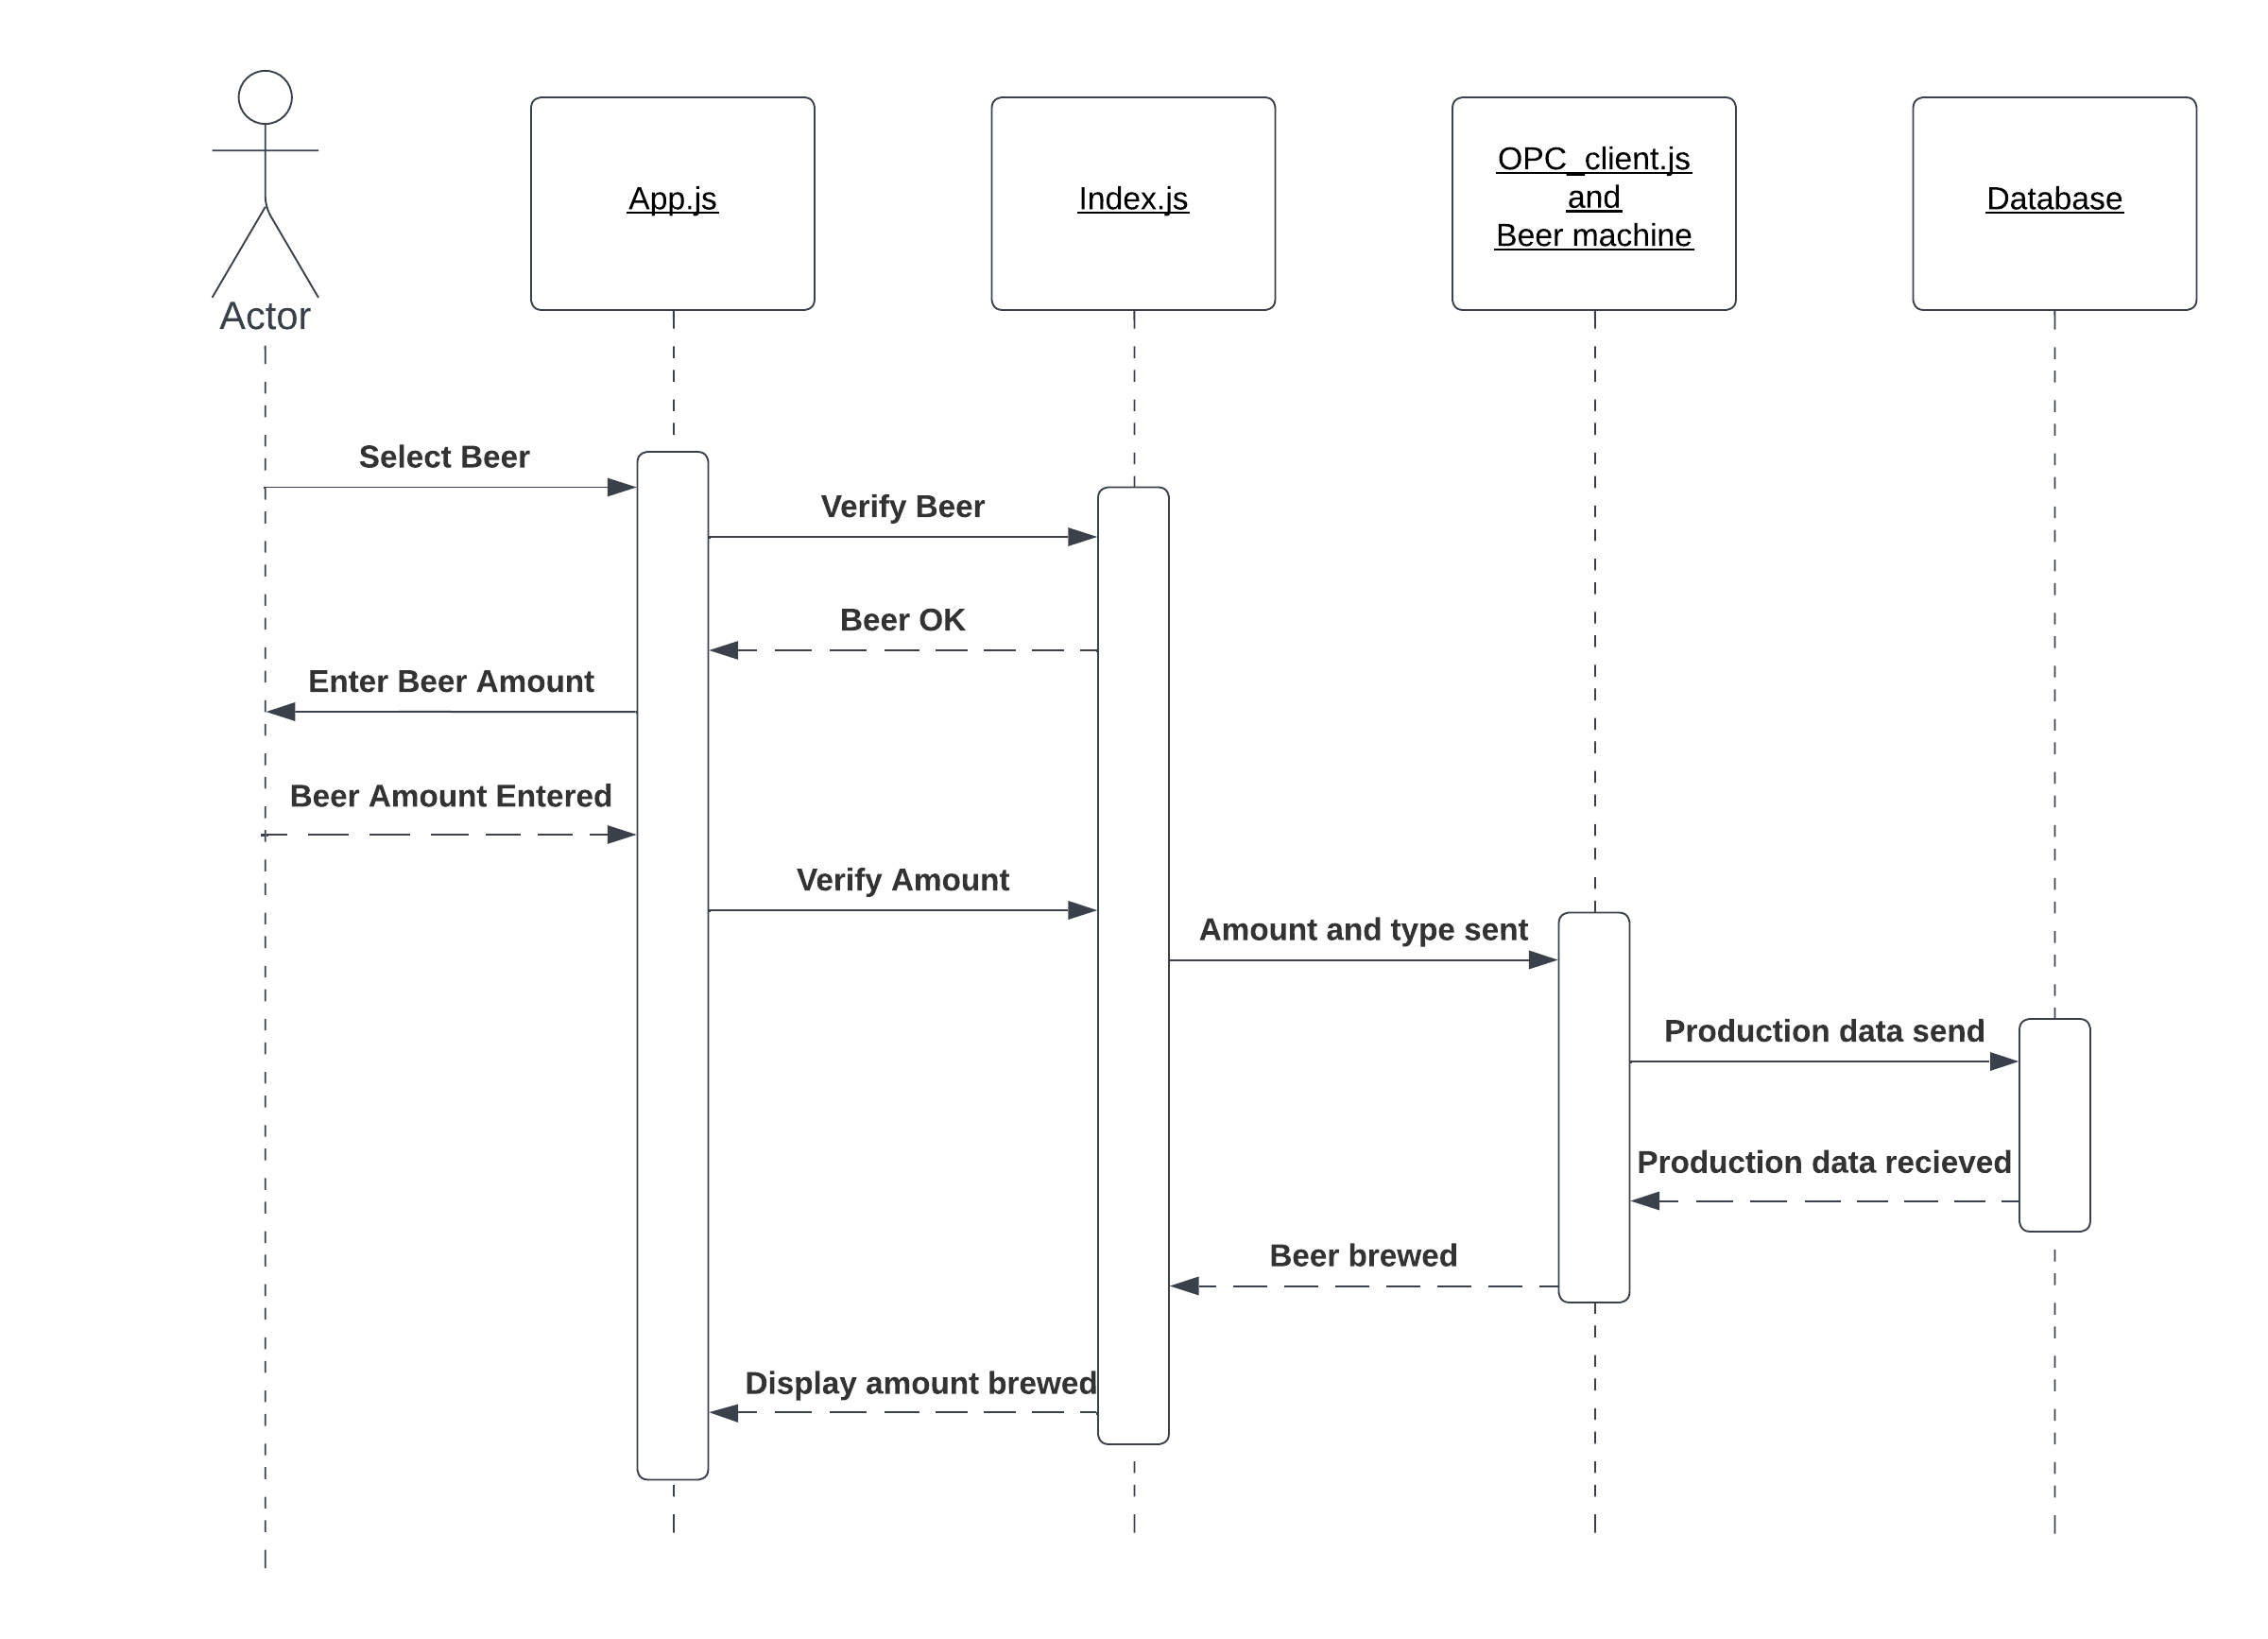
\includegraphics[width=1\textwidth]{img/SQdiagram_implementation.png}
        \caption{Sequence diagram of the system}
        \label{fig:SQdiagram_implementation}
    \end{figure}
\end{center}

Figure \ref{fig:SQdiagram_implementation} shows the sequence diagram of the system. The diagram shows the behaviour and workflow between the different compononents and how the react to input. When a user selects a beer from the user-friendly interface the frontend(App.js) it will send a request to the backend, where the backend will verify the selected beer, then the request is sent back to the fronted where the user can input the amount of beer he wants breewed. When the amount and type is selected, the brewing request is sent to the OPC or beer machine. 
When the brewing is done, the data for the given batch production will be sent to the database, with data about the succes of the brewing, failures and etc. This data can be handled if needed to help optimize the brewing process. The client does not get this message it work internally in our automated system. The service will sent a message to the backend saying the beer is done, here the backend sent a request to the frontend where it user get displayed the beer type and amount brewed is a success.
Overall this is a simple representation of the sytems workflow, but it helps indicate the progress from selecting a beer to actually getting the product.

\begin{center}
    \centering
    \begin{figure}[H]
        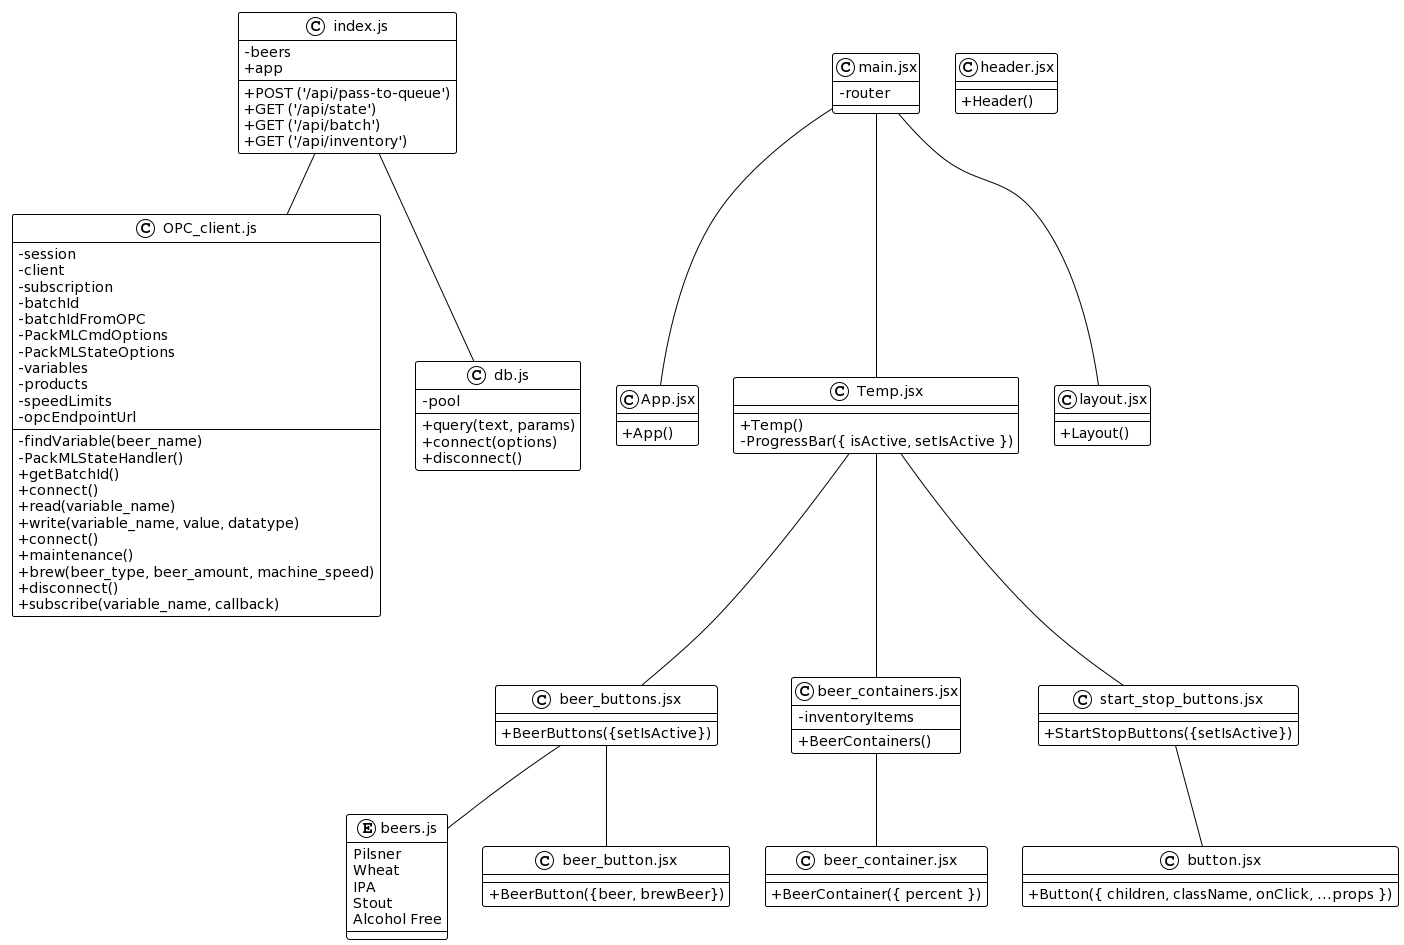
\includegraphics[width=1\textwidth]{img/class_diagram.png}
        \caption{Deployment diagram over the system}
        \label{fig:class_diagram}
    \end{figure}
\end{center}
Figure \ref{fig:class_diagram} shows the class diagram of the system. The diagram shows the different classes and how they are connected. The system is divided into three components, a dockerfile that boots up the backend, frontend and OPCUA-Client, we have the beer machine itself, and lastly the database which enables us to save data that is generated during the brewing process. This data collected can be accesed and help us udnerstand and give improvments to the system. \newline